% Options for packages loaded elsewhere
\PassOptionsToPackage{unicode}{hyperref}
\PassOptionsToPackage{hyphens}{url}
%
\documentclass[
  man]{apa6}
\usepackage{amsmath,amssymb}
\usepackage{lmodern}
\usepackage{iftex}
\ifPDFTeX
  \usepackage[T1]{fontenc}
  \usepackage[utf8]{inputenc}
  \usepackage{textcomp} % provide euro and other symbols
\else % if luatex or xetex
  \usepackage{unicode-math}
  \defaultfontfeatures{Scale=MatchLowercase}
  \defaultfontfeatures[\rmfamily]{Ligatures=TeX,Scale=1}
\fi
% Use upquote if available, for straight quotes in verbatim environments
\IfFileExists{upquote.sty}{\usepackage{upquote}}{}
\IfFileExists{microtype.sty}{% use microtype if available
  \usepackage[]{microtype}
  \UseMicrotypeSet[protrusion]{basicmath} % disable protrusion for tt fonts
}{}
\makeatletter
\@ifundefined{KOMAClassName}{% if non-KOMA class
  \IfFileExists{parskip.sty}{%
    \usepackage{parskip}
  }{% else
    \setlength{\parindent}{0pt}
    \setlength{\parskip}{6pt plus 2pt minus 1pt}}
}{% if KOMA class
  \KOMAoptions{parskip=half}}
\makeatother
\usepackage{xcolor}
\IfFileExists{xurl.sty}{\usepackage{xurl}}{} % add URL line breaks if available
\IfFileExists{bookmark.sty}{\usepackage{bookmark}}{\usepackage{hyperref}}
\hypersetup{
  pdftitle={The role of cognateness in non-native spoken word recognition},
  pdfkeywords={cognate, word recognition, translation, non-native,
spoken word recognition},
  hidelinks,
  pdfcreator={LaTeX via pandoc}}
\urlstyle{same} % disable monospaced font for URLs
\usepackage{graphicx}
\makeatletter
\def\maxwidth{\ifdim\Gin@nat@width>\linewidth\linewidth\else\Gin@nat@width\fi}
\def\maxheight{\ifdim\Gin@nat@height>\textheight\textheight\else\Gin@nat@height\fi}
\makeatother
% Scale images if necessary, so that they will not overflow the page
% margins by default, and it is still possible to overwrite the defaults
% using explicit options in \includegraphics[width, height, ...]{}
\setkeys{Gin}{width=\maxwidth,height=\maxheight,keepaspectratio}
% Set default figure placement to htbp
\makeatletter
\def\fps@figure{htbp}
\makeatother
\setlength{\emergencystretch}{3em} % prevent overfull lines
\providecommand{\tightlist}{%
  \setlength{\itemsep}{0pt}\setlength{\parskip}{0pt}}
\setcounter{secnumdepth}{-\maxdimen} % remove section numbering
\usepackage{amsmath}
\usepackage{booktabs}
\usepackage{caption}
\usepackage{longtable}
\ifLuaTeX
  \usepackage{selnolig}  % disable illegal ligatures
\fi
\newlength{\cslhangindent}
\setlength{\cslhangindent}{1.5em}
\newlength{\csllabelwidth}
\setlength{\csllabelwidth}{3em}
\newenvironment{CSLReferences}[2] % #1 hanging-ident, #2 entry spacing
 {% don't indent paragraphs
  \setlength{\parindent}{0pt}
  % turn on hanging indent if param 1 is 1
  \ifodd #1 \everypar{\setlength{\hangindent}{\cslhangindent}}\ignorespaces\fi
  % set entry spacing
  \ifnum #2 > 0
  \setlength{\parskip}{#2\baselineskip}
  \fi
 }%
 {}
\usepackage{calc}
\newcommand{\CSLBlock}[1]{#1\hfill\break}
\newcommand{\CSLLeftMargin}[1]{\parbox[t]{\csllabelwidth}{#1}}
\newcommand{\CSLRightInline}[1]{\parbox[t]{\linewidth - \csllabelwidth}{#1}\break}
\newcommand{\CSLIndent}[1]{\hspace{\cslhangindent}#1}

\title{The role of cognateness in non-native spoken word recognition}
\author{true \and true \and true \and true}
\date{}

\begin{document}
\maketitle
\begin{abstract}
There is compelling evidence that bilinguals access their lexicon in a
language non-selective way. For example, bilinguals produce and
translated cognates (words whose translation in the other language is
form-similar) faster than non-cognates, suggesting that the phonology of
both languages interact during word production and comprehension (Costa
et al., 2000; Christoffels et al., 2006). Previous literature on this
effect has often relied on measures of overall form-similarity to
categorise words into cognates andnon-cognates, such as the Levenshtein
distance. These measures partially ignore potential sources of
variability during lexical access like vowel vs.~consonant overlap,
overlap in stressed syllables, onset overlap or the distance in features
between both translations. In this study, we explored the impact of some
of these variables on non-native word translation task: Spanish and
English participants listened to non-native words (Catalan or Spanish)
and were prompted to type their translation in their native language.
Critically, participants where unfamiliar with the testing language,
ensuring that they were not able to translate words based on previous
knowledge on their meaning, leaving phonological information as the only
cue participants were able to exploit to translate words to their native
language correctly. We analysed the probability of correct translations,
adjusting for the amount of vowel overlap, consonant overlap, overlap at
stress position, overlap at onset, and distance in features between
replaced phonemes, including the average frequency of phonological
neighbours of the target words are a covariate.
\end{abstract}

\hypertarget{introduction}{%
\section{Introduction}\label{introduction}}

\hypertarget{non-native-language-comprehension-is-difficult-but-cognateness-helps}{%
\subsection{Non-native language comprehension is difficult, but
cognateness
helps}\label{non-native-language-comprehension-is-difficult-but-cognateness-helps}}

Humans are able to recognise spoken words without much effort, even in
adverse conditions such as compressed speech (De Haan 1982) or the loss
of segmental information (Warren 1970). But even in the most ideal of
the situations, the processes engaged in word recognition do not occur
without uncertainty. The speech input activates multiple candidate
lexical entries based on their similarity with the signal, and for word
recognition to take place, the lexical system must select one of the
candidates. There is extensive literature about how the number of
candidates, their frequency, and their phonological and semantic
similarity with the target word impacts the dynamics of word
recognition. However, less is known about how these factors affect the
recognition of words in a non-native language.

Listening to speech in a non-native language is more costly than doing
so in the native language, even if one is proficient in the non-native
language. The source of this increased cognitive effort is likely to
originate at multiple levels. For instance, some sounds in the speech
signal do not correspond to any phoneme in the native language,
segmenting the speech signal relies on previous familiarity with word
forms or with the statistical regularities of the language, or word
order might be different in both languages (e.g., subject-object-verb
vs.~subject-verb-object.). The listener, however, is rarely completely
naïve to the language they are listening to. All languages share, to
some extent, similarities, frequently due to their typological
closeness, which can be exploited by listeners of a non-native language.

Lexical similarity, for example, provides useful information to
sequential language learners. Romance language like Spanish, Italian,
French or Catalan, share many similarities at the lexical level in the
form of cognates (Schepens, Dijkstra, and Grootjen 2012). Cognates are
cross-language synonyms whose form (e.g., phonology, orthography,
signature) is similar. The cause of this similarity is frequently
attributed to a shared etymological origin. This is the case of
\emph{puerta} and \emph{porta} (\emph{door} in Spanish and Catalan,
respectively)\footnote{Some form-similar cross-language synonyms are
  technically not cognates. For example, \emph{sun} and \emph{sol} (in
  Spanish), share their phonological onset, but their etymology points
  to different origins. We will use the word \emph{cognateness} to
  include all form-similar cross-language synonyms for simplicity. It is
  highly implausible that etymology plays a direct role on language
  perception if it is not via form-similarity, since it is not necessary
  for participants in psycholinguistic experiments to be aware of the
  etymology of the words they encounter in the tasks to be subject to
  the effect of form-similarity.}. There is evidence that cognates are
learnt more easily in L2 than non-cognates. De Groot and Keijzer (2000)
presented 40 Dutch natives 60 pairs of translation equivalents. In each
learning trial, two words were presented in a screen side-by-side: one
in Dutch and one pseudoword. Pseudowords were generated in such way that
were easily pronounceable and were phonotactically legal in Dutch. Word
pairs varied in their form-similarity (number of shared letters,
40-70\%). Participants were tested twice in the same task with one week
of difference. Participants' performance was better for cognates across
both testing sessions, suggesting that cognates were learnt and retained
more easily than non-cognates. Converging evidence was provided by Lotto
and De Groot (1998) in Dutch natives learning Italian words: cognates
were learnt more easily than non-cognates.

Cognates are not only learnt faster than non-cognates, but also
translated faster. Early accounts of bilingual lexical access described
two possible routes for translating a word from L1 to L2 or \emph{vice
versa}: (1) via direct links between L1-L2 links or (2) through
word-concept links. Both translation routes are available during
translation (Potter et al. 1984; Kroll, Curley, and others 1988). These
models assumed that the strength of the word-concept associations in
both L1 and L2 is a function of their frequency of use, in order to
account for the influence of both the lexical frequency of the presented
word and the target word in translation tasks on participant's
performance. Under the assumption that bilinguals use L1 more often,
Kroll and Stewart (1994) proposed the asymmetric hypothesis, predicting
stronger word-concept associations between L1 representations compared
to L2 representations. This would make L2-to-L1 translation more reliant
to the direct translation route (L1-L2 association) than L1-to-L2
translation. This prediction has three consequences: (1) L2-to-L1
translation is expected to be faster than L1-to-L2 translation (as it
does not rely on conceptual mediation during translation), and (2) since
word-to-word connections (like the L1-L2 one) occurs at the lexical
level (and not at the conceptual level), it should be sensitive to the
form-similarity between both words, and therefore to cognateness, and
(3) since low-proficiency bilinguals rely more on the direct route
during translation, and this route is sensitive to cognateness, their
performance during backward translation tasks should not only be better
than during forward translation, but also enhanced by the cognate status
of L1 and L2 representations.

To test these predictions, Degroot, Dannenburg, and Vanhell (1994) and
Groot (1992) asked 52 Dutch natives with high (yet non-native) English
proficiency to translate words from either Dutch to English (forward
translation, L1 to L2) or from English to Dutch (backward translation,
L2 to L1). In each trial, participants were presented visually with a
word in English or Dutch, and were asked to speak out loud its
translation in the other language as soon as possible. The authors
reported three main findings: (1) reaction times and accuracy were
roughly equivalent in across both forward and backward conditions
(although slightly faster in the former), (2) semantic variables, such
as imageability, were positively associated with participants'
performance more strongly in the forward translation conditional,
although the effect size was small, (3) cognates were translated equally
fast in both conditions, but non-cognates were translated faster during
backward translation than during forward translation, and (4) when
translating cognates participants' performance across both conditions
was less sensitive to semantic variables than when translating
non-cognates. These results prompted the authors to reject a hard
version Kroll and Stewart (1994)'s asymmetric hypothesis, and suggest
that both conceptually mediated and direct translation routes are active
during translation, but backward translation relies more strongly on
direct links between L1 and L2 representations, which makes it more
sensitive to cognateness than forward translation. When the authors
tested a group of bilinguals with higher proficiency in English, their
results pointed in the same direction.

The idealised lexicon considered by the models describe above only
considers word-word connections between translation equivalents. More
recent studies have highlighted the role of the rich network of
connections that given word establishes with other phonologically or
conceptually related words. Collins and Loftus (1975) introduced this
notion into their theory of semantic processing, and later Luce and
Pisoni (1998) operationalised this dimension in their Neighbourhood
Activation Model (NAM). In this model, lexical selection is mediated not
only by the lexical frequency of the target word, and the number of
activated candidates, but also by the frequency of the candidates. Luce
and Pisoni (1998) designed a lexical decision task in which English
native participants listened to a word across several conditions of
noise-to-signal ratio. The authors then used a computerised lexicon to
calculate the number of phonological neighbours around each of the
presented words, based on phonetic similarity matrices, and the average
lexical frequency of such neighbourhoods. Participants answered more
faster and more accurately to high frequency words. Words from high
density neighbourhoods were responded to more accurately, but more
slowly. The average lexical frequency of the neighbourhood was
associated to a decrease in accuracy. Low frequency words were responded
to more accurately in low density neighbours than in high density
neighbours. The authors concluded that, although both word lexical
frequency and neighbourhood density can, in principle, facilitate spoken
word recognition, this effect was modulated by the frequency of the
neighbourhood: when phonological neighbours are more frequent, lexical
selection is hindered (Goldinger, Luce, and Pisoni 1989; Luce, Pisoni,
and Goldinger 1990).

The role of neighbourhood lexical frequency on bilingual spoken word
recognition is unclear. Across several modalities, bilinguals'
recognition of words in a language is affected by form-similarity and
frequency of words in the other language. The parallel activation
hypothesis accounts for this phenomenon, suggesting that lexical access
is language-non selective. There is strong evidence supporting this
claim in both comprehension, production, and translation, and across
modalities. Much of this evidence stems from the fact that bilinguals'
production times are faster when naming cognates (i.e., words whose
translation in the other language is form-similar) than non-cognates.
Both phonological and semantic links between translations underlie
facilitatory effect of cognateness. The activation of form-similar words
in the non-target language that do not share meaning with the target
word, however, interferes with lexical selection. Disentangling the
effect of semantic and phonological links during spoken word recognition
is challenging when participants are bilingual.

This has important implications to non-native word recognition: is word
recognition facilitated by cognateness via translation? The answer is
not straightforward. Disentangling the effect of form- and conceptual
similarity in a bilingual sample is daunting, given that second language
learners are able to exploit \ldots{}

In the present study, we used a fully monolingual sample to disentangle
the effect of neighbourhood frequency and phonological similarity. We
asked participants to translate word in a language they had no
significant experience with. This made sure that participants were
unaware of any semantic relationship between the (non-native) words they
heard and their translation, and could only rely on their phonological
similarity to guess their translation. We tested the role of the amount
of phonological similarity between the presented and the target words,
the lexical frequency of the target word, and the average lexical
frequency of the target word's phonological neighbourhood.

\hypertarget{methods}{%
\section{Methods}\label{methods}}

\hypertarget{participants}{%
\subsection{Participants}\label{participants}}

Data collection took place from June 04th, 2020 to June 28th, 2020. We
collected data from 104 participants (\emph{Mean} = 21.79 years,
\emph{SD} = 2.43, \emph{Min} = 18, \emph{Max} = 33). 72 participants
were British English native speakers living in United Kingdom (46), and
32 participants were Spanish native speakers living in Spain (27
female). Participants in UK were recruited via Prolific (5£
compensation) and SONA (compensation in academic credits). Participants
in Spain were contacted via announcements in Faculties, and were
compensated 5€ or an Amazon voucher for the same value. Participants
were asked to complete the experiment in a quiet place with good
internet connection. We excluded data from participants that a)
self-rated their oral and/or written skills in a second or third
language as higher than 4 in a 5-point scale (\emph{n} = 1), b) were
diagnosed with a language (\emph{n} = 2) , or c) did not contribute more
than 80\% of valid trials (\emph{n} = 9).

\hypertarget{procedure}{%
\subsection{Procedure}\label{procedure}}

The experiment was implemented online using Psychopy/Pavlovia (Peirce et
al. 2019). Participants accessed the study from a link provided by
Prolific or SONA and completed the experiment from a browser (Chrome or
Mozilla). Participants were informed about the aims of the study and
gave informed consent for participating. This experiment was Then,
participants answered a series of questions about their demographic
status, their language background, and the set up they were using for
completing the study. Third, participants completed the experimental
task. Participants were informed that they would listen to a series of
pre-recorded words in Catalan or Spanish (English participants) or only
Catalan (Spanish participants). They were instructed to listen to each
word, guess its meaning in English (English participants) or Spanish
(Spanish participants), and type their answer as soon as possible.
English participants were randomly assigned to the list of Catalan or
Spanish trials. Participants in the Catalan list were presented with 86
trials, and participants in the Spanish list were presented with 103
trials.

Each trial started with a yellow fixation point presented during one
second on the centre of the screen over a black background. After one
second, the audio started playing while the dot remained being displayed
until the audio ended. Upon the offset of the fixation point and audio,
participants were prompted to write their answer by a ``\textgreater{}''
symbol. Typed letters were displayed in the screen in real time to
provide visual feed-back to participants. Participants were allowed to
correct their answer. Then, participants pressed the RETURN key to start
and new trial. We excluded trials where participants did not type an
existing word in the correspondent language, or did not type anything at
all. Trials where the response was mistyped by only one character were
counted as correct, as long as the respond did not correspond to a
distinct word. Participants contributed a total of 8077 valid trials
(5235 in Catalan, 2842 in Spanish). The task took approximately 15
minutes to be completed.

\hypertarget{stimuli}{%
\subsection{Stimuli}\label{stimuli}}

Participants listened to one audio file in each trial. This audio file
corresponded to a word in Catalan (for Spanish speakers, and for English
participants allocated in the Catalan condition) or Spanish (for English
speakers allocated in the Spanish condition). The audio files were the
same ones used in child experiments conducted in the Laboratori de
Recerca en Infància of Universitat Pompeu Fabra (Barcelona, Spain).
These audio files were recorded by a proficient Catalan-Spanish female
bilingual from the Metropolitan Area of Barcelona in a child-directed
manner. Catalan and Spanish words were recorded at 44,100 Hz in separate
files in the same session, and then de-noised using Audacity and
normalised at peak intensity using Praat (Broersma and Weenink 2021).
The average duration of the audios was 1.20 (\emph{SD} = 0.18,
\emph{Min} = 0.78, \emph{Max} = 1.58). The average duration of the
Catalan audios was 1.23 seconds (\emph{SD} = 0.19, \emph{Min} = 0.80,
\emph{Max} = 1.58), and the average duration of the Spanish audios was
1.16 seconds (\emph{SD} = 0.15, \emph{Min} = 0.78, \emph{Max} = 1.53).
Table 1 summarises the lexical frequency, phonological neighbourhood
density and phonological overlap of the words included in the Catalan
and the Spanish lists.

\captionsetup[table]{labelformat=empty,skip=1pt}
\begin{longtable}{lrrrrrrrrrr}
\toprule
 & \multicolumn{2}{c}{\textbf{Frequency (per million)}} & \multicolumn{2}{c}{\textbf{Frequency (Zipf score)}} & \multicolumn{2}{c}{\emph{\textbf{PTHN}}} & \multicolumn{2}{c}{\textbf{Consonant similarity}} & \multicolumn{2}{c}{\textbf{Vowel similarity}} \\ 
 \cmidrule(lr){2-3} \cmidrule(lr){4-5} \cmidrule(lr){6-7} \cmidrule(lr){8-9} \cmidrule(lr){10-11}
 & Mean & \emph{SD} & Mean & \emph{SD} & Mean & \emph{SD} & Mean & \emph{SD} & Mean & \emph{SD} \\ 
\midrule
ENG-CAT & $46.80$ & $77.23$ & $4.31$ & $0.59$ & $3.26$ & $3.74$ & $0.34$ & $0.17$ & $0.17$ & $0.11$ \\ 
ENG-SPA & $43.91$ & $67.53$ & $4.32$ & $0.56$ & $3.52$ & $4.10$ & $0.34$ & $0.15$ & $0.14$ & $0.10$ \\ 
SPA-CAT & $53.32$ & $156.19$ & $4.23$ & $0.62$ & $1.62$ & $2.62$ & $0.42$ & $0.15$ & $0.27$ & $0.12$ \\ 
 \bottomrule
\end{longtable}

\hypertarget{data-analysis}{%
\subsection{Data analysis}\label{data-analysis}}

We modelled the probability of participants guessing the correct
translation of each input word using a generalised multilevel Bayesian
regression model with a Bernoulli logit link distribution. We first
fitted a base model (Model 0) that only included the lexical frequency
(\texttt{frequency}) of the target word as a fixed effect, with a random
intercept per participant. Second, we extended the model to include
\texttt{pthn} as a fixed effect, with a random slope by participant
(Model 1). Third, we added the fixed effect \texttt{consonant\_ratio}
and the \texttt{pthn:consonant\_ratio}, and random slopes for both
effects by participant (Model 2). Third, we added the fixed effect
\texttt{vowel\_ratio} and the \texttt{pthn:vowel\_ratio}, and random
slopes for both effects by participant (Model 3). Finally, we fit a
model that included the two-way interactions
\texttt{pthn:consonant\_ratio} and \texttt{pthn:vowel\_ratio}, an their
random slopes by participant (Model 4). Continuous predictors were
standardised and categorical predictors were sum-coded (Schad et al.
2020). Model 4 can be formally expressed as:

\$\$ \begin{align*}

&\textbf{Likelihood}  \\
y_{i} \sim& Bernoulli(p_{i}) && \text{[probability of correct translation]} \\ \\

&\textbf{Parameters}  \\

logit(p_{i}) = ~ &  \beta_{0[p,w]} ~ +  && \text{[linear model]}\\
& \beta_{1[p]} ~ Frequency_{i} ~ + \\
& \beta_{2[p]} ~ PTHN_i ~ + \\
& \beta_{3[p]} ~ Similarity_i ~ + \\
& \beta_{4[p]} ~ (PTHN_i \times Similarity_i) \\ \\

\beta_{0-6[p,w]} \sim& ~  \mathcal{N}(\mu_{\beta_{j}}, \sigma_{\beta_{j}}) \text{, for participant } p ~\text{in 1, ..., } P ~\text{and  word } w ~\text{in 1, ..., } W && \text{[participant- and word-level intercepts]} \\
\beta_{1-6[p]} \sim& ~  \mathcal{N}(\mu_{\beta_{j}}, \sigma_{\beta_{j}}) \text{, for participant } p ~\text{in 1, ..., } P
&& \text{[participant-level coefficients]} \\ \\

&\textbf{Prior}  \\

\mu_{\beta_{p,w}} ~ \sim& ~ \mathcal{N}(0, 3) && \text{[participant-level coefficients]} \\
\sigma_{\beta_{p}}, ~ \sigma_{\beta_{w}} \sim& ~ Cauchy(0, 3) && \text{[SD for population and participant]} \\
\rho_{p}, ~ \rho_{w} \sim& ~LKJ(5) && \text{[correlation between participant-level coefficients]} \\


\end{align*} \$\$

To test and account for cross-group differences, we included a random
intercept for each group. We compared models using leave-one-out
cross-validation (\emph{LOO}) (Vehtari, Gelman, and Gabry 2017). More
information about the models and model comparison can be found in
Appendix 2. All analyses were performed in R environment (RCore 2019).
We used the tidyverse family of R packages to process data and to
generate figures, and the brms R package (Bürkner 2017) using the
cmdstanr backend to the Stan probabilistic language (Carpenter et al.
2017) to estimate and compare the models (see Appendix 1 for mode
details on the models).

\hypertarget{results}{%
\section{Results}\label{results}}

All models showed good out-of-sample predictive validity, as suggested
by the fact that the expected log-probability density was many times
larger than its associated standard error. Model 4, which included all
main effects and the two-way interactions between PTHN and vowel
similarity, and PTHN and consonant similarity, showed the best
performance (see Table 2).

\captionsetup[table]{labelformat=empty,skip=1pt}
\begin{longtable}{lrrrrrr}
\toprule
 & \emph{\textbf{LOOELPD}} & \emph{\textbf{SE}} & \emph{\textbf{LOOIC}} & \textbf{\emph{SE}IC} & \emph{\textbf{LOOdiff}} & \emph{\textbf{SEdiff}} \\ 
\midrule
Model 3 & $-4,276.17$ & $45.33$ & $8,552.34$ & $90.66$ & - & - \\ 
Model 2 & $-4,293.17$ & $45.33$ & $8,586.34$ & $90.65$ & $-17.00$ & $6.40$ \\ 
Model 1 & $-4,308.60$ & $45.28$ & $8,617.19$ & $90.56$ & $-32.43$ & $9.07$ \\ 
Model 0 & $-4,319.55$ & $45.11$ & $8,639.10$ & $90.21$ & $-43.38$ & $10.34$ \\ 
 \bottomrule
\end{longtable}

We now report the mean of the posterior distribution of each coefficient
in Model 3, along with its associated measures of uncertainty. For
interpretability, we transformed the estimates of the intercept using
the inverse logit function so that the values are expressed in
probability of correct response instead of log-odds, and we transformed
the coefficients of the rest of predictors divided by four. Dividing a
coefficient expressed in log-odds by four returns an approximate of the
derivative of the logistic function indicating the maximum steepness of
the logistic curve. This way, the coefficients are expressed as
increases/decreases in probability of correct translation (Gelman, Hill,
and Vehtari 2020).

\begin{figure}
\centering
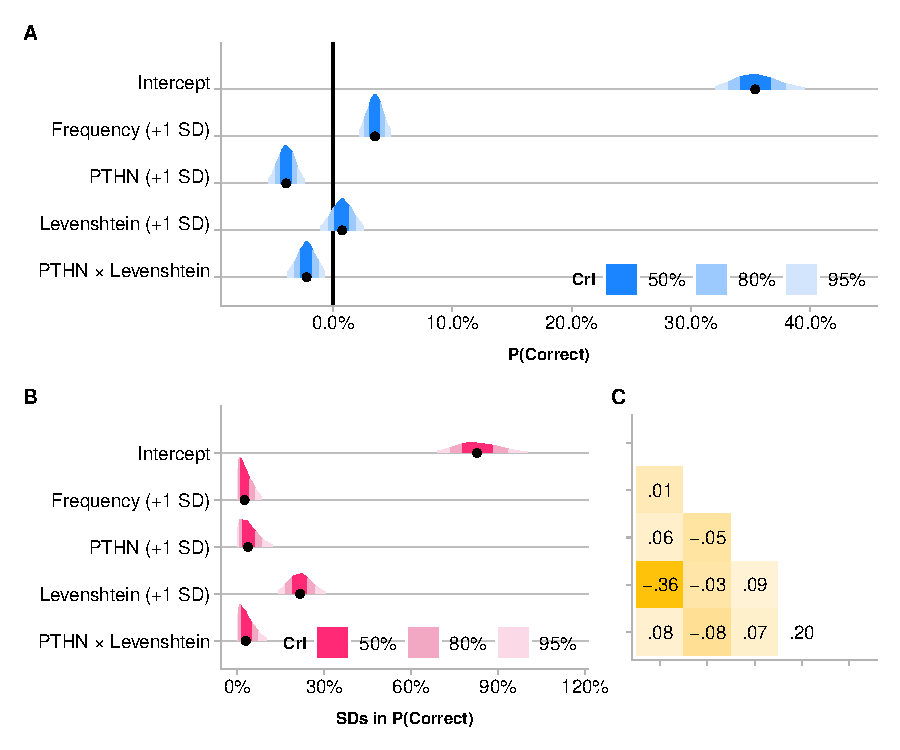
\includegraphics{manuscript_files/figure-latex/posterior_fix-1.pdf}
\caption{Estimated posterior distributions of coefficients in Model 3.
A) Population-level effects. Distributions indicate the estimated
posterior likelihood density of each coefficient. Credible intervals
(CrI), represented with increasingly lighter segmentents in the
distribution indicate the range of values that contain the true value
with 95\%, 80\%, and 50\%, given the data we have collected. Points
represent the mean of the distribution. The intercept has been
transformed using the inverse logit to get the average probability of
correct response. The rest of the coefficients have been transformed
using the divide-by-four rule to get the maximum change in probability
of correct response associated with a unit increase in each predictor
variable. B) Participant-level coefficient variability. Our model
estimated participant-level coefficients to account for the dependency
between responses from the same participant. Distributions in this panel
indicate the estimated variability across coefficients from different
participants, expressed as standard deviations (SD). C) Correlation
between participant-level effects. Our model allowed participant-level
coefficients to co-vary. This panel represents the Pearson correlations
between each pair of coefficients, expressed as the mean of the
posterior distribution of each correlation. Coefficients are represented
in the X- and Y-axis in the same order as indicated in the Y-axis of
panels A and C.}
\end{figure}

Overall, participants were 25.03\%, (\emph{SE} = 56.22\%, 95\%
\emph{CrI} = {[}56.22\%, 56.22\%{]}) likely to produce correct
translations. Every standard deviation increment in the translation's
lexical frequency (\emph{SD} = 0.59) increased the probability of a
correct responses in 3.90\% (\emph{SE} = 0.98\%, 95\% \emph{CrI} =
{[}0.98\%, 0.98\%{]}). The number of the translation's more frequent
phonological neighbours, on the other hand, decreased the probability of
a correct responses in -4.60\% (\emph{SE} = -1.15\%, 95\% \emph{CrI} =
{[}-1.15\%, -1.15\%{]}) for every increase in 1 \emph{SD} (3.65). The
effect of phonological similarity was conditional to the phonological
density of the translation. Phonological similarity barely increased the
probability of a correct responses (3.05\%, \emph{SE} = 1\%, 95\%
\emph{CrI} = {[}0.76\%, 1\%{]}) by itself. However, for every \emph{SD}
increase in PTHN, phonological similarity increased in -2\%, (\emph{SE}
= -0.62\%, 95\% \emph{CrI} = {[}-0.62\%, -0.62\%{]}) such probability.

\begin{figure}
\centering
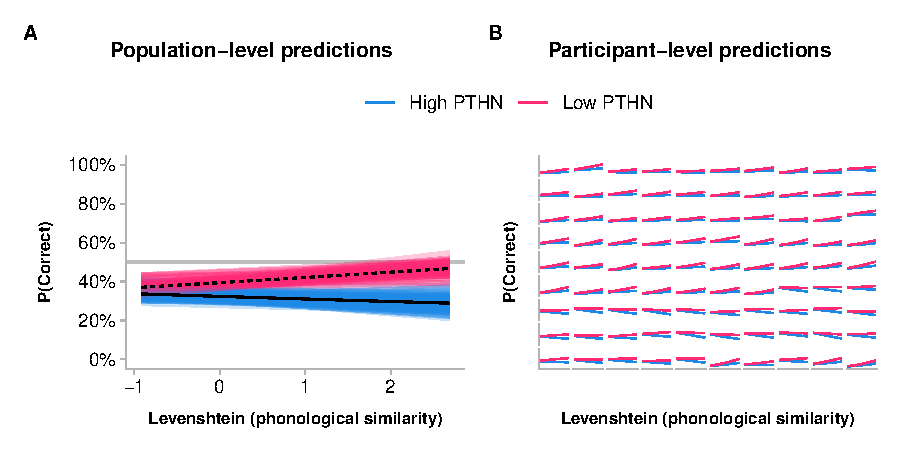
\includegraphics{manuscript_files/figure-latex/marginal_effects-1.pdf}
\caption{Expected mean posterior predictions.}
\end{figure}

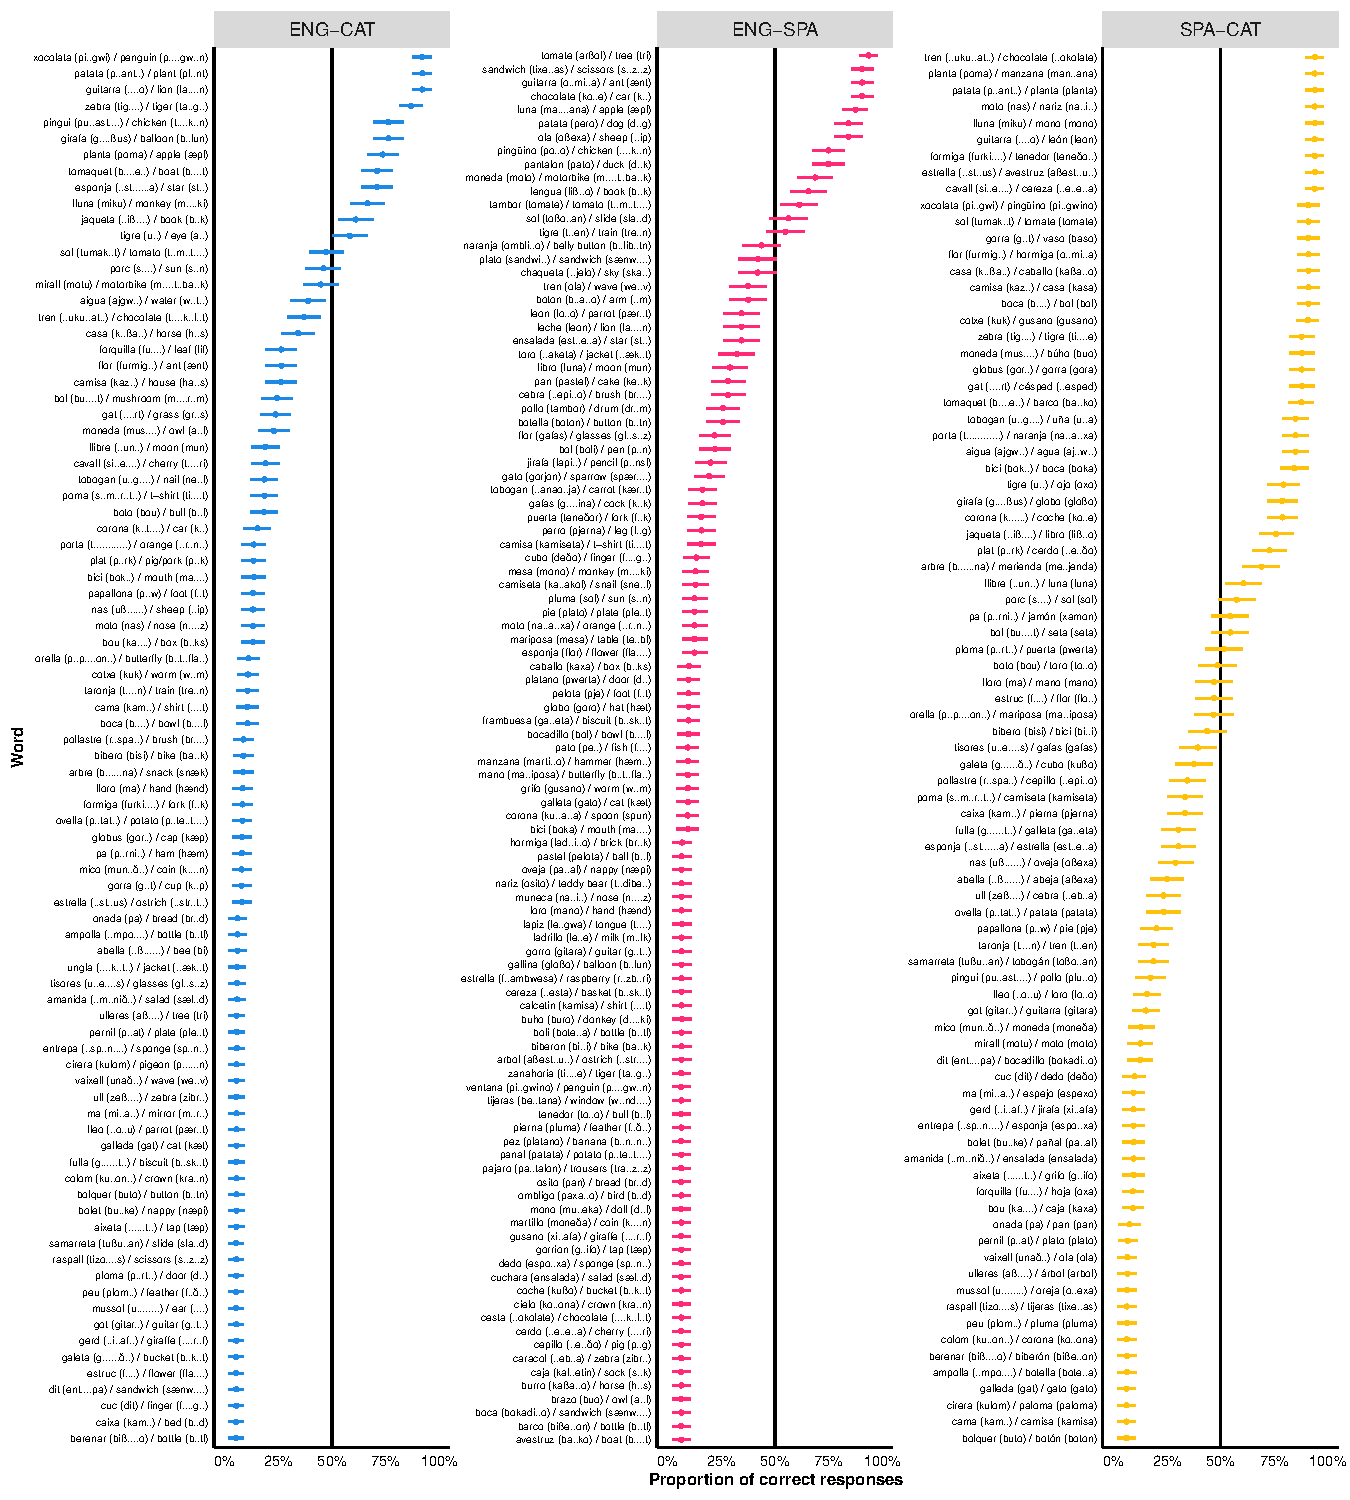
\includegraphics{manuscript_files/figure-latex/accuracy-1.pdf}

\hypertarget{discussion}{%
\section{Discussion}\label{discussion}}

\newpage

\hypertarget{references}{%
\section{References}\label{references}}

\begingroup
\setlength{\parindent}{-0.5in}
\setlength{\leftskip}{0.5in}

\hypertarget{refs}{}
\begin{CSLReferences}{1}{0}
\leavevmode\vadjust pre{\hypertarget{ref-broersma2021praat}{}}%
Broersma, Paul, and David Weenink. 2021. {``Praat: Doing Phonetics by
Computer {[}Computer Program{]}.''} \url{http://www.praat.org/}.

\leavevmode\vadjust pre{\hypertarget{ref-burkner2017brms}{}}%
Bürkner, Paul-Christian. 2017. {``Brms: An r Package for Bayesian
Multilevel Models Using Stan.''} \emph{Journal of Statistical Software}
80 (1): 1--28.

\leavevmode\vadjust pre{\hypertarget{ref-carpenter2017stan}{}}%
Carpenter, Bob, Andrew Gelman, Matthew D Hoffman, Daniel Lee, Ben
Goodrich, Michael Betancourt, Marcus A Brubaker, Jiqiang Guo, Peter Li,
and Allen Riddell. 2017. {``Stan: A Probabilistic Programming
Language.''} \emph{Grantee Submission} 76 (1): 1--32.

\leavevmode\vadjust pre{\hypertarget{ref-collins1975spreading}{}}%
Collins, Allan M, and Elizabeth F Loftus. 1975. {``A
Spreading-Activation Theory of Semantic Processing.''}
\emph{Psychological Review} 82 (6): 407.

\leavevmode\vadjust pre{\hypertarget{ref-de2000hard}{}}%
De Groot, Annette MB, and Rineke Keijzer. 2000. {``What Is Hard to Learn
Is Easy to Forget: The Roles of Word Concreteness, Cognate Status, and
Word Frequency in Foreign-Language Vocabulary Learning and
Forgetting.''} \emph{Language Learning} 50 (1): 1--56.

\leavevmode\vadjust pre{\hypertarget{ref-de1982relationship}{}}%
De Haan, Henry J. 1982. {``The Relationship of Estimated
Comprehensibility to the Rate of Connected Speech.''} \emph{Perception
\& Psychophysics} 32 (1): 27--31.

\leavevmode\vadjust pre{\hypertarget{ref-degroot1994forward}{}}%
Degroot, Annette MB, Lucia Dannenburg, and Janet G Vanhell. 1994.
{``Forward and Backward Word Translation by Bilinguals.''} \emph{Journal
of Memory and Language} 33 (5): 600--629.

\leavevmode\vadjust pre{\hypertarget{ref-gelman2020regression}{}}%
Gelman, Andrew, Jennifer Hill, and Aki Vehtari. 2020. \emph{Regression
and Other Stories}. Cambridge University Press.

\leavevmode\vadjust pre{\hypertarget{ref-goldinger1989priming}{}}%
Goldinger, Stephen D, Paul A Luce, and David B Pisoni. 1989. {``Priming
Lexical Neighbors of Spoken Words: Effects of Competition and
Inhibition.''} \emph{Journal of Memory and Language} 28 (5): 501--18.

\leavevmode\vadjust pre{\hypertarget{ref-de1992determinants}{}}%
Groot, Annette M de. 1992. {``Determinants of Word Translation.''}
\emph{Journal of Experimental Psychology: Learning, Memory, and
Cognition} 18 (5): 1001.

\leavevmode\vadjust pre{\hypertarget{ref-kroll1988lexical}{}}%
Kroll, Judith F, Janet Curley, and others. 1988. {``Lexical Memory in
Novice Bilinguals: The Role of Concepts in Retrieving Second Language
Words.''} \emph{Practical Aspects of Memory} 2 (389-395): 8.

\leavevmode\vadjust pre{\hypertarget{ref-kroll1994category}{}}%
Kroll, Judith F, and Erika Stewart. 1994. {``Category Interference in
Translation and Picture Naming: Evidence for Asymmetric Connections
Between Bilingual Memory Representations.''} \emph{Journal of Memory and
Language} 33 (2): 149--74.

\leavevmode\vadjust pre{\hypertarget{ref-lotto1998effects}{}}%
Lotto, Lorella, and Annette MB De Groot. 1998. {``Effects of Learning
Method and Word Type on Acquiring Vocabulary in an Unfamiliar
Language.''} \emph{Language Learning} 48 (1): 31--69.

\leavevmode\vadjust pre{\hypertarget{ref-luce1998recognizing}{}}%
Luce, Paul A, and David B Pisoni. 1998. {``Recognizing Spoken Words: The
Neighborhood Activation Model.''} \emph{Ear and Hearing} 19 (1): 1.

\leavevmode\vadjust pre{\hypertarget{ref-luce1990similarity}{}}%
Luce, Paul A, David B Pisoni, and Steven D Goldinger. 1990.
{``Similarity Neighborhoods of Spoken Words.''}

\leavevmode\vadjust pre{\hypertarget{ref-peirce2019psychopy2}{}}%
Peirce, Jonathan, Jeremy R Gray, Sol Simpson, Michael MacAskill, Richard
Höchenberger, Hiroyuki Sogo, Erik Kastman, and Jonas Kristoffer
Lindeløv. 2019. {``PsychoPy2: Experiments in Behavior Made Easy.''}
\emph{Behavior Research Methods} 51 (1): 195--203.

\leavevmode\vadjust pre{\hypertarget{ref-potter1984lexical}{}}%
Potter, Mary C, Kwok-Fai So, Barbara Von Eckardt, and Laurie B Feldman.
1984. {``Lexical and Conceptual Representation in Beginning and
Proficient Bilinguals.''} \emph{Journal of Verbal Learning and Verbal
Behavior} 23 (1): 23--38.

\leavevmode\vadjust pre{\hypertarget{ref-rcore2019r}{}}%
RCore, TEAM. 2019. {``R: A Language and Environment for Statistical
Computing. R Foundation for Statistical Computing, Austria.''}

\leavevmode\vadjust pre{\hypertarget{ref-schad2020capitalize}{}}%
Schad, Daniel J, Shravan Vasishth, Sven Hohenstein, and Reinhold Kliegl.
2020. {``How to Capitalize on a Priori Contrasts in Linear (Mixed)
Models: A Tutorial.''} \emph{Journal of Memory and Language} 110:
104038.

\leavevmode\vadjust pre{\hypertarget{ref-schepens2012distributions}{}}%
Schepens, Job, Ton Dijkstra, and Franc Grootjen. 2012. {``Distributions
of Cognates in Europe as Based on Levenshtein Distance.''}
\emph{Bilingualism: Language and Cognition} 15 (1): 157--66.

\leavevmode\vadjust pre{\hypertarget{ref-vehtari2017practical}{}}%
Vehtari, Aki, Andrew Gelman, and Jonah Gabry. 2017. {``Practical
Bayesian Model Evaluation Using Leave-One-Out Cross-Validation and
WAIC.''} \emph{Statistics and Computing} 27 (5): 1413--32.

\leavevmode\vadjust pre{\hypertarget{ref-warren1970perceptual}{}}%
Warren, Richard M. 1970. {``Perceptual Restoration of Missing Speech
Sounds.''} \emph{Science} 167 (3917): 392--93.

\end{CSLReferences}

\endgroup

\end{document}
